\newif \iftheory 

\theorytrue %\theoryfalse

\newif \ifblind

\blindtrue \blindfalse

\newcommand{\eli}[1]{\textcolor{blue}{[Eli: #1]}}
\newcommand{\meg}[1]{\textcolor{red}{[Megumi: #1]}}
\newcommand{\hannah}[1]{\textcolor{magenta}{[Hannah: #1]}}


% ~~~~~ Modify inside here ~~~~~%
\newcommand{\authorlist}{
% Author 1
Megumi Ando\iftheory\thanks{Computer Science Department, Tufts University, {\tt mando@cs.tufts.edu}}\fi
\and 
% Author 2
Anna Lysyanskaya\iftheory\thanks{Computer Science Department, Brown University, {\tt anna@cs.brown.edu}}\fi
\and 
% Author 3
Hannah Marsh\iftheory\thanks{Computer Science Department, Tufts University, {\tt hmarsh03@cs.tufts.edu}}\fi
\and
% Author 3
Eli Upfal\iftheory\thanks{Computer Science Department, Brown University, {\tt eli@cs.brown.edu}}\fi
}

\newcommand{\institutelist}{}


\newcommand{\titlelist}{\iftheory\begin{bf}\fi
% title
Onion Routing on Sparse Mix-Networks
\iftheory\end{bf}\fi}

% Path to stylefiles
\newcommand{\pathstyles}{./stylefiles}

% Path to preambles
\newcommand{\pathpreambles}{./preambles}

% Path to bibfiles
\newcommand{\pathbibs}{./bibfiles}

% ~~~~~ Modify inside here ~~~~~%


\iftheory
% PLAIN ARTICLE
\documentclass[11pt]{article}

% LNCS (DEFAULT)
\else
%\documentclass[envcountsame, 10pt]{\pathstyles/llncs}
\documentclass[runningheads,a4paper]{llncs}
\ifblind 
\institute{}
\else
\institute{\institutelist}
\fi
\fi

\ifblind 
\author{}
\else
\author{\authorlist} 
\fi
\pagestyle{plain}

\title{\titlelist}

% PREAMBLE
% PREAMBLE
\usepackage[utf8]{inputenc}
\usepackage{amsfonts}
\usepackage{amssymb}
\usepackage{circuitikz}
\usepackage{cite}

\usepackage{xcolor}
\usepackage[
	n,
	operators,
	advantage,
	sets,
	adversary,
	landau,
	probability,
	notions,	
	logic,
	ff,
	mm,
	primitives,
	events,
	complexity,
	asymptotics,
	keys]{cryptocode}
\usepackage{enumitem}
\setlist{nosep}
\usepackage[hidelinks]{hyperref}
%\usepackage{todonotes}

\usepackage{lscape}
\usepackage{mathtools}

% MACROS

% ~~ General

%\DeclareMathOperator*{\argmax}{arg\,max}
%\DeclareMathOperator*{\argmin}{arg\,min}

\renewcommand{\secpar}{\lambda}
\renewcommand{\secparam}{1^\lambda}


% ~~ Formatting
\definecolor{hybrid}{HTML}{0076BA}

\usepackage{caption} 
\captionsetup[table]{skip=10pt}


% ~~~ Begin document ~~~ %
\begin{document}

\maketitle
\iftheory
\thispagestyle{empty}
\fi

% ABSTRACT
\vspace{-8mm}
\begin{abstract}

Onion routing is a practical and widely used method for establishing anonymous communication channels. It works by routing ``onions'' through a mixnet of intermediaries, where each onion is formed by wrapping a private message in multiple layers of encryption. As these messages traverse the network, it becomes harder for an adversary to trace them back to their original senders. In previous work~\cite{ICALP:AndLysUpf18}, it was shown that statistical privacy can be achieved against the passive adversary when each intermediary is chosen uniformly at random from all nodes. However, this requires a complete network topology where the number of direct connections between servers grows quadratically, $O(n^2)$, with the size of the network. 

In this paper, we investigate a scalable alternative that offers comparable anonymity while only requiring $O(n)$ network edges. We propose $\Pi_x$, a new protocol that assumes an \textit{expander} topology---a class of graphs known for their strong connectivity despite being sparse. With this setup, each mix-node has its own probability distribution (based on its limited connections to other nodes) that clients sample from to determine the next hop in a routing path. We show that if these distributions are configured to resemble an expander graph, our protocol can match the anonymity guarantees of a fully connected mixnet, making it a more suitable choice for large-scale communication networks.


\iftheory
\vfill
%\noindent\textbf{Keywords:} 
%Keyword, 
%keyword, 
%keyword.
\fi
\end{abstract}
 

% ~~~ BODY ~~~ %
\iftheory
\newpage
\thispagestyle{empty}
\tableofcontents
\newpage
\setcounter{page}{1}
\fi

\newcommand{\parties}{\mathsf{Parties}}
\newcommand{\keygen}{\mathsf{KeyGen}}
\newcommand{\formonion}{\mathsf{FormOnion}}
\newcommand{\proconion}{\mathsf{PeelOnion}}
\newcommand{\proconionhelper}{\mathsf{PeelOnionHelper}}
\newcommand{\bruiseonion}{\mathsf{BruiseOnion}}
\newcommand{\polylog}{\mathsf{polylog}}
\newcommand{\early}{\mathsf{early}}
\newcommand{\late}{\mathsf{late}}
\newcommand{\recipient}{\mathsf{Recipient}}
\newcommand{\Bad}{\mathsf{Bad}}

\section{Introduction}

Protecting user privacy in communication is a growing challenge in modern networks. Anonymous communication channels are essential for preventing adversaries from linking users to their activities, whether it's for online privacy, whistleblowing, or secure voting. One well-known method for achieving anonymous communication is \textit{onion routing}, where messages are wrapped in layers of encryption and routed through a series of intermediaries, called mix-nodes, before reaching the intended recipient. Each intermediary decrypts a single layer, revealing only the next node in the chain and the ciphertext to forward. As an onion passes through the mixnet, it becomes increasingly difficult for an adversary to trace it back to the original sender. 

Onion routing is widely adopted due to its simplicity and ability to tolerate failures in a subset of mix-nodes. Systems like Tor, which implement onion routing, are used by millions of people daily to protect their online activities. However, despite its widespread use, the security guarantees of onion routing are not fully understood, especially in the face of powerful adversaries.

Previous work, such as the protocol $\Pi_p$ introduced in~\cite{ICALP:AndLysUpf18}, shows that \textit{statistical privacy} can be achieved against a passive adversary if the intermediaries in the mixnet are chosen uniformly at random from all available nodes in a fully connected network. However, this approach relies on a complete graph, where every node can communicate directly with every other node, leading to a quadratic increase in the number of network edges as the system scales to accommodate more mixnodes. Thus the fully connected mixnet is inefficient for large systems.

We present the design, implementation, and evaluation of $\Pi_x$, a new protocol that aims to provide similar levels of anonymity while requiring significantly fewer network edges. Instead of relying on a fully connected mixnet, $\Pi_x$ assumes an \textit{expander} topology, a class of sparse graphs that maintain strong connectivity even with very few edges. In our approach, each mix-node has a probability distribution based on its connections to a fixed number of other nodes, from which clients select the next hop in their routing path. We demonstrate that, by configuring these distributions to approximate an expander graph, $\Pi_x$ can provide the same anonymity guarantees as a fully connected network but with only $O(n)$ edges.

Through the design and evaluation of $\Pi_x$, we demonstrate that expander graphs can be a practical foundation for large-scale anonymous communication systems, providing a balance between efficiency and privacy.

\subsection{Progression of Goals}

In our exploration of onion routing protocols on an expander topology, we begin with the foundational settings introduced in~\cite{ICALP:AndLysUpf18}, which assumes a synchronous communication model where all messages are delivered within fixed rounds. The goal is to achieve statistical privacy against the network and passive adversaries, and differential privacy against the active adversary. We first aim to generalize these results to an expander topology. 

However, a practical challenge of this adaption is enabling efficient onion formation for senders without requiring full knowledge of the network topology, which may change between and even within a single execution of the protocol. In the first results of this paper, clients need to download and maintain the global network structure to select routing paths. However, this becomes impractical as the network scales. To address these issues, we propose a novel protocol extension: wrapping onions. In this approach, the client forms an initial onion with partial routing information and sends it to the first intermediary node. This node peels the first layer to reveal the next destination node, but because the graph is an expander, there may not be a direct link. Instead, the intermediary node must create a detour path to the next hop, wrapping the onion in additional layers, and forwarding it onward. By delegating some of the routing decisions to intermediary nodes, the protocol significantly reduces the burden on clients, as they no longer need to download or maintain the entire network topology. This wrapping mechanism also aligns well with the expander graph's natural properties, where efficient routing can be achieved with localized knowledge.

Another advantage of this approach becomes evident when the network experiences churn, where nodes and edges are dynamically added or removed during execution. In a static topology, an onion formed at the start of the protocol could potentially die at some point if a node goes offline. However, in the wrapping onions protocol, the responsibility for routing dynamically shifts to intermediary nodes, which are better positioned to adapt to local changes in the network. This makes the protocol inherently more robust to churn, as local routing decisions can reflect the current network state.

In summary, our progression starts by generalizing the provable guarantees of $\Pi_p$ and $\Pi_a$ to an expander graph topology, then we build on this foundation with the wrapping onions protocol, which enhances scalability by minimizing client-side network requirements and improves computational efficiency.


\section{Definitions}

\subsection{Security Parameter}

The security parameter\footnote{It is worth noting that ``$\lambda$'' is also commonly used to denote eigenvalues (of a graph's adjacency matrix). To avoid confusion, we will explicitly specify whenever $\lambda$ represents something other than the security parameter.}, $\lambda \in \mathbb{N}$, is a tunable input that quantifies a system's level of security. It can be adjusted to achieve various trade-offs (e.g., privacy vs. latency), since many system parameters and metrics are bound asymptotically by functions of $\lambda$. 

A function $f : \mathbb{N} \rightarrow \mathbb{R}$ is negligible in $\lambda$, written $f(\lambda) = \negl$, if for every polynomial~$p(\cdot)$ and all sufficiently large $\lambda$, 
$$
f(\lambda) < \frac{1}{p(\lambda)}.
$$
An event occurs with overwhelming probability if it is the complement of an event with probability negligible in $\lambda$. We say that two families of distributions~$\{D_{0, \lambda}\}_{\lambda \in\mathbb{N}}$ and $\{D_{1, \lambda}\}_{\lambda \in\mathbb{N}}$ are statistically close if the statistical distance between $D_{0, \lambda}$ and $D_{1, \lambda}$ is negligible in $\lambda$~\footnote{When the security parameter is clear by context, we abbreviate this notion by $D_0 \approx_s D_1$.}.

\subsection{Network and Participants}

Our setup requires two distinct roles: $N$ clients (users), who wish to send private messages to other clients, and a network of $n$ relays (mixnodes) that serve as intermediaries to unlink sender-receiver pairs. While each client has a direct connection to every relay, we model the mixnet of relays as an $r$-regular, $\beta$-expander graph, where all relays are assumed to be synchronized. In our definitions, $N$ is polynomially bounded by the security parameter $\lambda$. Additionally, the size of the mixnet, $n$, is bounded by: $O\left(\frac{N}{log^2 \lambda}\right)$. 

Each input to a protocol $\Pi$ is represented as an $N$-dimensional vector. When the protocol is executed on an input $\sigma = (\sigma_1, \dots, \sigma_N)$, each $\sigma_i$ consists of a collection of properly formed message pairs. A message pair $(m,j) \in \sigma_i$ represents user $i$'s intention to send message $m$ to user $j$. Let $\mathcal{M}$ denote the (bounded) message space. Then $(m,j)$ is considered properly formed if $m \in \mathcal{M}$ and $j \in [N]$. 

Let $\mathcal{M}(\sigma)$ represent the set of all messages in $\sigma$. It is defined as the multiset of all message pairs across all users' inputs, given by

$$
\mathcal{M}(\sigma_1, \dots, \sigma_N) = \bigcup_{i=1}^{N} \{ (m,j) \in \sigma_i \}.
$$

\subsection{Threat Model}

Let $\Pi$ be a protocol, and let $\sigma$ be a vector of inputs to $\Pi$. Given an adversary $\mathcal{A}$, the view $\mathsf{V}^{\Pi,\mathcal{A}}(\sigma)$ of $\mathcal{A}$ consists of all the information observable by the adversary while participating in $\Pi$ on input $\sigma$, possibly with additional randomness used by the adversary to make its decisions. Given an adversary $\mathcal{A}$, the output $\mathsf{O}^{\Pi,\mathcal{A}}(\sigma) = (\mathsf{O}^{\Pi,\mathcal{A}}_1(\sigma), \dots, \mathsf{O}^{\Pi,\mathcal{A}}_N(\sigma))$ of $\Pi$ on input $\sigma$ is a vector of outputs for the $N$ parties.

We consider the following standard adversary models, listed in increasing order of capability:

\begin{itemize}
    \item \textbf{Network adversary.} A network adversary can observe the bits flowing over every link in the network. If data is encrypted in an idealized scenario, the only information that a network adversary has is the \textit{volume} of traffic flowing over edges in the network.)\\
    
    \item \textbf{Passive adversary.} In addition to the capabilities of a network adversary, a passive adversary can monitor the internal states and operations of a constant fraction of the relays. The adversary selects which relays to monitor non-adaptively, meaning the choice is made before the protocol begins and remains fixed throughout execution. Importantly, we assume the passive adversary has full knowledge of the network topology to inform their selection of whom to monitor.\\
    
    \item \textbf{Active adversary.} In addition to the capabilities of a passive adversary, an active adversary can corrupt the behavior of a constant fraction of the relays. While the selection of whom to corrupt remains non-adaptive (and may be informed by the network topology), the behavior of corrupted parties can be altered on the fly. This includes deviating arbitrarily from the protocol (e.g., dropping, delaying, or repeating onions). \\
\end{itemize}

\subsection{Privacy Definitions}

We define the security of a communications protocol as the difficulty for the adversary to infer who is communicating with whom (beyond what is leaked from captured messages). Below, we introduce two flavors of security notions. We will show that our constructions achieve either statistical privacy or $(\epsilon,\delta)$-differential privacy~\cite{TCC:DMNS06} in the idealized encryption setting.\\

\begin{definition} [Statistical privacy] \label{def:statistical-privacy}
    Let $\Sigma^*$ be the input set consisting of every input of the form
    $$
    \sigma = \{(m_1, \pi(1)), \dots, (m_N, \pi(N))\},
    $$
    where $m_1, \dots, m_N \in \mathcal{M}$ and $\pi : [N] \rightarrow [N]$ is any permutation function over the set $[N]$. A communications protocol $\Pi$ is statistically private from the adversaries in the class $\mathcal{A}$ if, for all $\mathcal{A} \in \mathcal{A}$ and for all $\sigma_0, \sigma_1 \in \Sigma^*$ that differ only on the honest parties' inputs and outputs, the adversary's views $\mathsf{V}^{\Pi,\mathcal{A}}(\sigma_0)$ and $\mathsf{V}^{\Pi,\mathcal{A}}(\sigma_1)$ are statistically indistinguishable, i.e.,
    $$
    \Delta(\mathsf{V}^{\Pi,\mathcal{A}}(\sigma_0), \mathsf{V}^{\Pi,\mathcal{A}}(\sigma_1)) = \mathsf{negl}(\lambda),
    $$
    where $\lambda \in \mathbb{N}$ denotes the security parameter, and $\Delta(\cdot, \cdot)$ denotes the statistical distance (i.e., the total variation distance). Protocol $\Pi$ is perfectly secure if the statistical distance is 0.
    \eli{variation distance - but there are no probabilities here??}\\
    \hannah{Each $\mathsf{V}^{\Pi,\mathcal{A}}(\sigma)$ is a probability distribution. We get statistical privacy if dropping Alice's onion vs. not dropping her onion produce probability distributions that are statistically close.}
\end{definition}

\begin{definition} [Distance between inputs] \label{def:distance-between-inputs} 
    The distance between two inputs $\sigma_0 = (\sigma_1, \dots, \sigma_N)$ and $\sigma_1 = (\sigma_1', \dots, \sigma_N')$, denoted $d(\sigma_0, \sigma_1)$, is given by
    $$
    d(\sigma_0, \sigma_1) \overset{\Delta}{=} \sum_{i=1}^{N} |\sigma_{i} \vartriangle \sigma_{i}'|,
    $$
    where $\vartriangle$ represents the symmetric difference between $\sigma_{i}$ and $\sigma_{i}'$.\\
\end{definition}

\begin{definition} [Neighboring inputs] \label{def:neighboring-inputs} 
    Two inputs $\sigma_0$ and $\sigma_1$ are neighboring if 
    $$
    d(\sigma_0, \sigma_1) \leq 1.
    $$\\
\end{definition}

\begin{definition} [$(\epsilon, \delta)$-DP~\cite{TCC:DMNS06}] \label{def:dp}
    A communication protocol $\Pi$ is $(\epsilon, \delta)$-differentially private if for every adversary $\adv$ and every pair of neighboring inputs $\sigma_0$ and $\sigma_1$ and every set $\mathcal{V}$ of adversarial views, 
    \[
    \prob{\mathsf{View}^{\Pi, \adv}(\sigma_0) \in \mathcal{V}} \le e^\epsilon \prob{\mathsf{View}^{\Pi, \adv}(\sigma_1) \in \mathcal{V}} + \delta .
    \]
    
    While differential privacy is defined with respect to neighboring inputs, it also provides (albeit weaker) guarantees for non-neighboring inputs; it is known that the security parameters degrade proportionally with the distance between the inputs~\cite{TCC:DMNS06}.

    We say that $\Pi$ is computationally $(\epsilon,\delta)$-differentially private~\cite{C:MPRV09} if the above bound holds for all polynomially bounded adversaries.\\
\end{definition} 

\subsection{Performance Metrics}

\begin{definition} [Correctness] \label{def:correctness}
    We define correctness with respect to passive adversaries since message delivery cannot be guaranteed in the presence of an active adversary.
    \eli{we need appropriate definition for active adversary}\\
    
    A communications protocol $\Pi$ is said to be correct on an input $\sigma \in \Sigma$ if for any passive adversary $\mathcal{A}$, and for every recipient $j \in [N]$, the output $\mathsf{O}^{\Pi, \mathcal{A}}_j(\sigma)$ corresponds to the multiset of all messages for recipient $j$ in the input vector $\sigma$. That is,
    $$
    \mathsf{O}^{\Pi, \mathcal{A}}_j(\sigma) = \{m \mid (m, j) \in \mathcal{M}(\sigma)\},
    $$
    where $\mathcal{M}(\sigma)$ denotes the multiset of all messages in $\sigma$. \\
\end{definition}

\begin{definition} [Communication complexity blow-up] \label{def:ccb}
    The communication complexity blow-up of an OR protocol $\Pi$ is defined with respect to an input vector $\sigma$ and an adversary $\mathcal{A}$. 
    
    Denoted $\gamma^{\Pi, \mathcal{A}}(\sigma)$, it is the expected ratio between the total number $\Gamma^{\Pi, \mathcal{A}}(\sigma)$ of onions transmitted in protocol $\Pi$ and the total number $\mathcal{M}(\sigma)$ of messages in the input vector. That is,
    $$
    \gamma^{\Pi, \mathcal{A}}(\sigma) \overset{\Delta}{=} \mathbb{E} \left[ \frac{\Gamma^{\Pi, \mathcal{A}}(\sigma)}{|\mathcal{M}(\sigma)|} \right].
    $$

    $\gamma^{\Pi, \mathcal{A}}(\sigma)$ essentially measures how many more onion transmissions are required by the protocol, compared with transmitting the messages in onions directly from the senders to the recipients (without passing through intermediaries). We assume that every message $m \in \mathcal{M}$ in the message space $\mathcal{M}$ “fits” into a single onion. The communication complexity is measured in unit onions, which is appropriate when the parties pass primarily onions to each other.\\
\end{definition}

\begin{definition} [Server load] \label{def:serverload}
    The server load of an OR protocol $\Pi$ is defined with respect to an input vector $\sigma$ and an adversary $\mathcal{A}$. It is the expected number of onions processed by a single party in a round.\\
\end{definition}

\begin{definition} [Latency] \label{def:latency}
    The latency of an OR protocol $\Pi$ is defined with respect to an input vector $\sigma$ and an adversary $\mathcal{A}$. It is the expected number of rounds in a protocol execution.
    
    Protocols with having low (i.e., polynomial in the security parameter) server load, low communication complexity blow-up, and low latency are considered efficient OR protocols.\\
\end{definition}

\newpage

\subsection{Properties of Expander Graphs}

Expander graphs are a class of sparse graphs where any subset of its vertices remains well-connected to the rest of the graph, making them particularly useful in the design of network protocols.

\begin{definition} [$\beta$-expander] \label{def:beta-expander}
    Formally, a graph $G = (V, E)$ is called a $\beta$-expander if, for every subset of vertices $S \subset V$ where $|S| \leq |V|/2$, the number of edges leaving $S$ (denoted by $\texttt{out}(S)$) satisfies:
    
    $$
    |\texttt{out}(S)| \geq \beta \cdot |S|.
    $$
    
    In other words, the number of edges connecting $S$ to its complement $V \setminus S$ is proportional to the size of $S$, so that that even small subsets of the graph are well-connected, as visualized in Fig.~\ref{fig:beta-expander}\\

    \begin{figure}
        \centering
        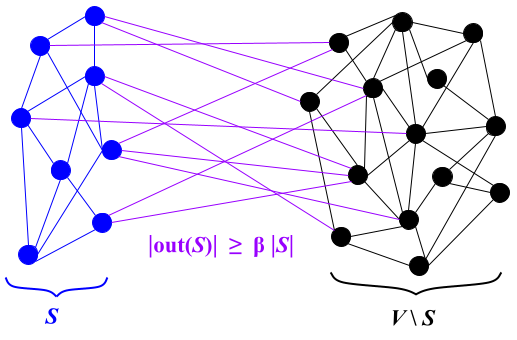
\includegraphics[width=0.5\textwidth]{template/figures/Expander graph.png}
        \caption{A graph $G = (V, E)$ is said to be a $\beta$-expander if the number of edges connecting any minority subset of vertices $S \subset V$ to its complement $V \setminus S$, denoted $|\texttt{out}(S)|$, is at least $\beta |S|$.}
        \label{fig:beta-expander}
    \end{figure}

\end{definition}

\begin{definition} [$\lambda$-absolute eiganvalue expander] \label{def:eiganvalue-expander}
     An $r$-regular graph $G = (V, E)$ is called a $\lambda$-absolute eiganvalue expander if, $|\lambda_2|,|\lambda_3|,...,|\lambda_n| \leq \lambda$. Here, $|\lambda_1| \geq |\lambda_2| \geq ... \geq |\lambda_n|$ are the eiganvalues of the adjacency matrix $A$ of $G$.\\

     In fact, iff $G$ is an $r$-regular $\beta$-expander, for some constant $\beta$, then it is also a $\lambda$-absolute eiganvalue expander where $\lambda = r - \frac{\beta^2}{2r}$ (from \textit{Cheeger's inequality})
     \eli{it's an iff}.
\end{definition}

\subsubsection{Random Walks} 
    
A \textit{random walk} on a graph is a process where, starting from an initial node, a ``walker'' moves to a neighboring node at each step according to some probability distribution over the neighbors of the current node. 

\begin{definition} [Simple random walk] \label{def:simp-random-walk}
    In a \textit{simple random walk} on a graph $G = (V, E)$, the walker starts at some vertex $v_0 \in V$. Let $\Gamma(v)$ denote the set of neighbors for each vertex $v \in V$. At each time step, the walker moves to a randomly chosen neighbor of the current vertex, where each neighbor is selected with equal probability. More formally, let $X_t$ denote the position of the walker at time $t$. The transition probability from vertex $v$ to vertex $u$ is given by:
    
    $$
    P(X_{t+1} = u \mid X_t = v) =
    \begin{cases}
    \frac{1}{|\Gamma(v)|} & \text{if } (v, u) \in E, \\
    0 & \text{otherwise}.
    \end{cases}
    $$
    
    Thus, at each step, the walker moves to one of the neighbors of the current vertex with equal probability.
\end{definition}

An important property is that a random walk on an expander graph rapidly converges to a uniform distribution, meaning that after a few \eli{polylog in the network size} \hannah{Isn't it \textit{logarithmic} in the number of nodes?} steps, the probability of being at any given vertex becomes nearly uniform, regardless of the starting point.

\begin{definition} [Stationary distribution] \label{stationary-distribution}
    The \textit{stationary distribution} of a random walk is a probability distribution over the vertices such that if the walker is distributed according to this distribution at some time $t$, it will have the same distribution at time $t+1$. For a connected, non-bipartite graph, the random walk converges to a unique stationary distribution, and for regular graphs, this stationary distribution is uniform over all vertices.
\end{definition}

The rate of convergence to this stationary distribution in an expander graph is closely tied to the \textit{second-largest eigenvalue} of their adjacency matrix. 

\begin{definition} [Second-largest eigenvalue] \label{def:second-largest-eig}
    Let $\lambda_1 \geq \lambda_2 \geq \cdots \geq \lambda_n$ be the eigenvalues of the adjacency matrix of a $r$-regular graph. The largest eigenvalue $\lambda_1$ is equal to $r$, and the second-largest eigenvalue $\lambda_2$ (or the spectral gap $\lambda_1 - \lambda_2$) determines how quickly the random walk on the graph mixes. Specifically, the mixing time is inversely proportional to the spectral gap. A smaller value of $\lambda_2$ indicates faster mixing.

For a strong expander, the second-largest eigenvalue $\lambda_2$ satisfies:

$$
\lambda_2 \leq 1 - \epsilon
$$

for some constant $\epsilon > 0$. This indicates that the graph has good expansion properties, meaning that the random walk mixes rapidly. In our protocol $\Pi_x$, we take advantage of these properties of $\beta$-expanders, which allows us to prove that the routing paths chosen for onions will sufficiently mix after a polylogarithmic number of steps.
\end{definition}



\clearpage


\section{Our Protocol}

As previously established, our problem setting consists of $N$ clients (users) and $n$ relays (mixnodes). While each client has a direct connection to every relay, we model the mixnet of relays as an $r$-regular, $\beta$-expander graph.

Each client begins with a single message they wish to send privately to another client. We assume that the set of intended recipients is a permutation of the senders, meaning that each client sends and receives exactly one message. At the start of the protocol, clients must download the current state of the network, which they use to construct a valid routing path through the mixnet. To bootstrap a path, a client selects the first hop uniformly at random from the set of all relays. The remaining path is then constructed by performing a random walk of fixed length $L$. Finally, the recipient is appended, resulting in a path of length $L + 1$ that traverses randomly through the mixnet and terminates at the intended recipient.

The client can then use this path to encrypt their message in successive layers. The innermost layer contains the message encrypted under the recipient’s public key, and each additional layer (added in reverse order of the path) specifies the next hop. Consequently, the innermost layer can only be received and decrypted by the recipient if all preceding layers are properly ``peeled'' by the mixnodes in the selected path.

At the beginning of the first round, each client sends their formed onion to the first hop. In subsequent rounds, each relay decrypts the outermost layer and then forwards the peeled onion accordingly.

In the final round, the recipient can then reveal the original message.


\subsection{Network Adversary}
\begin{theorem} \label{clm:network}
    $\Pi_x$ is statistically private from the network adversary when $\frac{N}{n} = \Omega(\log^2 \lambda)$, and $L = \Omega(\log^2 \lambda)$, where $\lambda \in \mathbb{N}$ denotes the security parameter.\\
\end{theorem}
\eli{$\lambda$ is both eigenvalue and security parameter.}
\begin{proof} [Proof of Theorem~\ref{clm:network}]

    We proceed by induction. In the first round, the adversary knows the exact location of every sender's onion. Let $O$ represent one of these onions. We aim to show that after a polylogarithmic number of rounds, the adversary's belief about which onion is $O$ becomes indistinguishable from a uniform distribution across all $N$ onions.\\
    
    Fix a round $i$. Because of mixing occurring at each relay, all onions emerging from a given relay this round will have the same probability of being $O$ (from the adversary’s perspective). Let $S = \{ s_1, \dots, s_n \}$ denote the set of all relays, sorted by the average probability of onions emerging from them. Without loss of generality, assume $n$ is even, allowing us to partition $S$ into two groups, $S_1 = \{ s_1,..., s_{\frac{n}{2}} \}$ and $S_2 = \{ s_{\frac{n}{2} + 1},..., s_n \}$.\\

    Let $G_1$ and $G_2$ represent the total probability mass of onions routed this round to relays in $S_1$ and $S_2$, respectively. From Chernoff bounds for Poisson trials (need lemma), with overwhelming probability, the average server loads for each of $S_1$ and $S_2$ will be arbitrarily close to the expected value ($\frac{N}{n}$). It follows that the difference in the sizes of $G_1$ and $G_2$ is negligible, and thus $G_1$ represents approximately the top $\frac{N}{2}$ most likely onions to be $O$'s while $G_2$ represents the rest. \\
    
    Now denote $X_1$ and $X_2$ as the highest and lowest probabilities in $G_1$ and let $X_2$ and $X_3$ be the highest and lowest probabilities in $G_2$. Let $o_1$ and $o_4$ be the most probable and least probable onions next round with probabilities $x_1$ and $x_4$, respectively. Let $R_1$ and $R_2$ represent the relays that $o_1$ and $o_4$ were routed to in round $i + 1$. From the properties of expander graphs, we know there are at least $\frac{\beta n}{2}$ edges connecting $S_1$ and $S_2$. Given that the total number of edges in the graph is $\frac{nr}{2}$, we can expect $G_2$ to contribute on average $\frac{\beta N}{r n} = \Omega(\log^2 \lambda)$ onions to $R_1$ and similarly, $G_1$ contributes $\frac{\beta N}{r n} = \Omega(\log^2 \lambda)$ onions to $R_2$. From Chernoff bounds for Poisson trials (Lemma ~\ref{lem:chernoff-1}), with overwhelming probability, $G_1$ and $G_2$ contribute to $R_1$ and $R_2$ a number of onions arbitrarily close to these expected numbers. Thus for every $d > 0$,
    $$
    x_1 = Pr[o_1] \leq \left( 1 - \frac{\beta}{r} + d \right) \cdot X_1 + \left(\frac{\beta}{r} - d \right) \cdot X_3
    $$
    $$
    x_4 = Pr[o_4] \geq \left( 1 - \frac{\beta}{r} + d \right) \cdot X_4 + \left(\frac{\beta}{r} - d \right) \cdot X_2
    $$

    Taking the difference:
    $$
    x_1 - x_4 \leq \left( 1 - \frac{\beta}{r} \right) ( X_1 - X_4) + \left(\frac{\beta}{r} \right) (X_3 - X_2) + d ( X_1 + X_2 - X_3 - X_4 )
    $$
    $$
    \leq \left( 1 - \frac{\beta}{r} \right) ( X_1 - X_4) + 2d ( X_1 - X_4 )
    $$
    $$
    = \left( 1 - \frac{\beta}{r} + 2d \right) ( X_1 - X_4)
    $$

    In particular, for all $0 < d <\frac{\beta}{2r}$:
    $$
    \left( 1 - \frac{\beta}{r} + 2d \right) < 1
    $$

    Therefore, the gap between the highest and lowest probabilities is reduced by at least a constant fraction every round. Thus after a polylogarithmic number of rounds, the gap becomes negligible. By partitioning the onions into an appropriately large number ($\Omega(1)$) of groups, we can show that $\Pi_x$ achieves statistical privacy after $L = \Omega(\log^2 \lambda)$ rounds. \\
    \eli{the general argument is correct but the proof is not complete. The differences are not , but within some parameter that should be added to the calculation. We also need to sum the error probabilities for all the events. }

\end{proof}

\subsection{Passive Adversary}

\begin{theorem} \label{clm:passive}
    $\Pi_x$ is statistically private against a passive adversary who can monitor up to a constant fraction $\chi < \frac{1}{2}$ of the servers. Assume $\frac{N}{n} = \Omega(\log^2 \lambda)$ and $L = \Omega(\frac{1}{\log^2 \lambda)}$, where $\lambda \in \mathbb{N}$ represents the security parameter.\\
\end{theorem}

\begin{proof} [Proof of Theorem~\ref{clm:passive}]

We prove this by induction. Similar to the network adversary setup, in the first round, the adversary knows the exact location of each sender’s onion. Let $O$ denote one such onion. Due to mixing occurring at the $(1 - \chi)n$ honest relays, onions emerging from an honest party in any given round have the same probability of being $O$ from the adversary's perspective. However, onions emitted by a corrupted relay carry the same likelihood of being $O$ as they had the last time they were mixed at an honest party. Until an onion encounters an honest hop, it has probability 0 (except for $O$, with 1).\\

The challenger reveals a sequence of rounds $i_{s, 1} < i_{e, 1} < i_{s, 2} < i_{e, 2} < \dots < i_{s, L} < i_{e, L} \le r$ where $O$ was mixed by an honest relay. Here, each cycle, $(i_{s, j}, \dots, i_{e, j})$, starts and ends with ``good hops'' (where $O$ mixes with other onions) and may include a constant number of “bad hops” in between (where $O$ does not mix). For each cycle $(i_{s, j}, \dots, i_{e, j})$, the challenger informs the adversary that $O$ belongs to a set $\mathcal{O}_{s, j}$ of approximately $(1 - \chi)N$ onions emerging from honest relays at hop $i_{s, j}$. It also reveals that $O$ will not mix again until hop $i_{e, j}$. Let $S$ represent the set of honest relays to which the onions in $\mathcal{O}_{s, j}$ are routed to in round $i_{s, j}$, sorted by the probability of onions after they are mixed. We partition $S$ into two groups: $S_1 = \{ s_1,..., s_{\frac{(1 - \chi)n}{2}} \}$ and $S_2 = \{ s_{\frac{(1 - \chi)n}{2} + 1},..., s_{(1 - \chi)n} \}$.\\

Let $G_1$ and $G_2$ represent the total probability mass of onions routed to relays in $S_1$ and $S_2$, respectively. By applying Chernoff bounds for Poisson trials, we find that, WHP, the average server loads for each of $S_1$ and $S_2$ are arbitrarily close to the expected value, $\frac{N}{n}$. Consequently, the difference in sizes between $G_1$ and $G_2$ is negligible, meaning $G_1$ contains approximately the top half most likely onions in $\mathcal{O}_{s, j}$ to be $O$, while $G_2$ contains the rest.\\

Define $X_1$ and $X_2$ as the highest and lowest probabilities in $G_1$ and let $X_3$ and $X_4$ represent the highest and lowest probabilities in $G_2$. Let $o_1$ and $o_4$ denote the most and least probable onions routed to honest relays in round $i_{e, j}$, with probabilities $x_1$ and $x_4$, respectively. Let $R_1$ and $R_2$ be the next honest relays $o_1$ and $o_4$ are routed to, with cycle lengths $c_1$ and $c_4$ for each. \\

From properties of expander graphs, we know that of all paths of length $c$ originating in $S_2$, a fraction $\frac{(1 - \chi)^2 r^c}{\beta^c}$ will end at $R_1$. Thus since $c = O(1)$, $G_2$ contributes an expected $\frac{(1 - \chi)^2 r^{c}}{\beta^{c}} \cdot \frac{N}{n} = \Omega(\log^2 \lambda)$ onions to $R_1$. Similarly, $G_1$ contributes $\Omega(\log^2 \lambda)$ onions to $R_2$. Applying Chernoff bounds, we find that $G_1$ and $G_2$ contribute onions to $R_1$ and $R_2$ in numbers close to these expectations. \\

It follows from the same logic in Thm.~\ref{clm:network} that the gap between the highest and lowest probabilities of onions at honest relays during any given round diminishes by at least $\frac{(1 - \chi)^2 r^{c}}{\beta^{c}}$ every round. Therefore, after a polylogarithmic number of rounds, this difference becomes negligible. By partitioning the onions into a sufficiently large number of groups ($\Omega(1)$), we conclude that $\Pi_x$ achieves statistical privacy against the passive adversary after $L = \Omega(\log^2 \lambda)$ rounds.
    
\end{proof}

% \begin{theorem}
%     $\Pi_x$ is statistically private from the passive adversary capable of monitoring up to a constant fraction $\chi < \frac{1}{2}$ of the servers when $\frac{N}{n} = \Omega(\log^2 \lambda)$, and $L = \Omega(\log^2 \lambda)$, where $\lambda \in \mathbb{N}$ denotes the security parameter.    
% \end{theorem}

% \begin{proof}
%     Let $\sigma_0$ and $\sigma_1$ represent two input vectors, and let $d(\sigma_0, \sigma_1)$ denote the distance between them. We aim to show that the adversary's views of $\sigma_0$ and $\sigma_1$ become indistinguishable after a polylogorithmic number of rounds.\\\\
%     We proceed with a proof by cases.\\
    
%     \begin{enumerate}[label=\textbf{\Roman*.}]
%         \item $d(\sigma_0, \sigma_1) \leq 2$:
        
%         In this case, $\sigma_1$ and $\sigma_0$ are the same except there may be a pair of onions, say $o_1$ and $o_2$, that were swapped. However, since each onion was routed to at least $\Omega(\log^2 \lambda)$ honest relays, it follows from Thm.~\ref{clm:network} that the gap between $o_1$ and $o_2$'s probabilities becomes negligible by end of the protocol. Thus, the adversary cannot distinguish between $\sigma_0$ and $\sigma_1$, and statistical privacy is achieved.\\
    
%         \item $d(\sigma_0, \sigma_1) > 2$:
        
%         Since $N = \mathsf{poly}(\lambda)$, we know the distance between $\sigma_0$ and $\sigma_1$ is also polynomial with respect to $\lambda$. Then we can reduce the problem to a series of smaller steps, each of which is equivalent to the first case, where $d(\sigma_0, \sigma_1)$ is at most 2. By applying the result from Case 1 iteratively (for a polynomial number of steps), we conclude that the adversary's views on $\sigma_0$ and $\sigma_1$ will become statistically indistinguishable after $\Omega(\log^2 \lambda)$ rounds.\\
%     \end{enumerate}
    
%     Thus $\Pi_x$ is statistically private against a passive adversary.
    
% \end{proof}

\subsection{Active Adversary}

While $\Pi_x$ is statistically private from the passive adversary, it is only differentially private against the active adversary. We describe the protocol by the setup and routing algorithms for every sender $i \in [n]$. Assume that $F$ is a pseudorandom function (PRF) and that each honest sender runs the same algorithms.\\

\textbf{\textit{Setup.}} During the setup phase, sender $i \in [n]$ prepares a set of onions from its input. For every message pair $u = \{m, j\}$ in $i$'s input, $i$ picks a sequence $T^u_1, \dots, T^u_L$ of servers by performing a random walk across the graph starting at some bootstrap node $T^u_1$, which is chosen uniformly at random from all servers in $[N]$. For all $\ell > 1$, each $T^u_\ell$ is chosen independently and uniformly at random from all neighbors of $T^u_{\ell - 1}$. $i$ then forms an onion from the message $m$, the routing path $(T^u_1, \dots, T^u_L, j)$, the public keys $(\text{pk}_{T^u_1}, \dots, \text{pk}_{T^u_L}, \text{pk}_j)$, and a list of empty nonces. Additionally, party $i$ forms some dummy onions (determined by the output of pseudorandom function $F$) as follows:\\

\begin{enumerate}
    \item \textbf{for} every server $k \in [N]$:
    \begin{enumerate}
        \item compute $b \leftarrow F(sk_{i,k}, \text{session}, 0)$, where $\text{session} \in \mathbb{N}$ denotes the protocol instance.
        \item \textbf{if} $b \equiv 1$ — set to occur with frequency $\frac{\alpha \log^2 \lambda}{N}$ for some constant $\alpha > 0$:\\
        --- \textbf{do}:
        \begin{enumerate}
            \item perform a random walk $T_1 = \{T_{1,1}, \dots, T_{1, \frac{L}{2} - 1}\}$, where $T_{1,1}$ is chosen uniformly at random from all neighbors of $k$. 
            \item perform a random walk $T_2 = \{T_{2,1}, \dots, T_{2, \frac{L}{2} - 1}\}$, where $T_{2,1}$ is chosen uniformly at random from all neighbors of $k$. 
            \item reverse the order of the nodes in $T_1$, forming $T^{\text{rev}}_1$.
            \item choose a receiver $j \in [n]$ chosen uniformly at random from all clients.
            \item create a new list $T = T^{\text{rev}}_1 \circ \{ k \} \circ T_2 \circ j$ which is of length $L + 1$, has server $k$ positioned at index $\frac{L}{2}$, and ends at a random client receiver $j$.
            \item create a list of $L$ nonces $s$, where $s_{\frac{L}{2}} = F(\text{checkpt}, F(sk_{i,k}, \text{session}, 1))$, and all other elements are $\bot$.
            \item form a dummy onion using the message $\bot$, the routing path $T$, the public keys associated with $T$, and the list $s$ of nonces.
        \end{enumerate}
        \item \textbf{end for}
    \end{enumerate}
    \item \textbf{end for}\\\\
 \end{enumerate}

 \begin{center}
    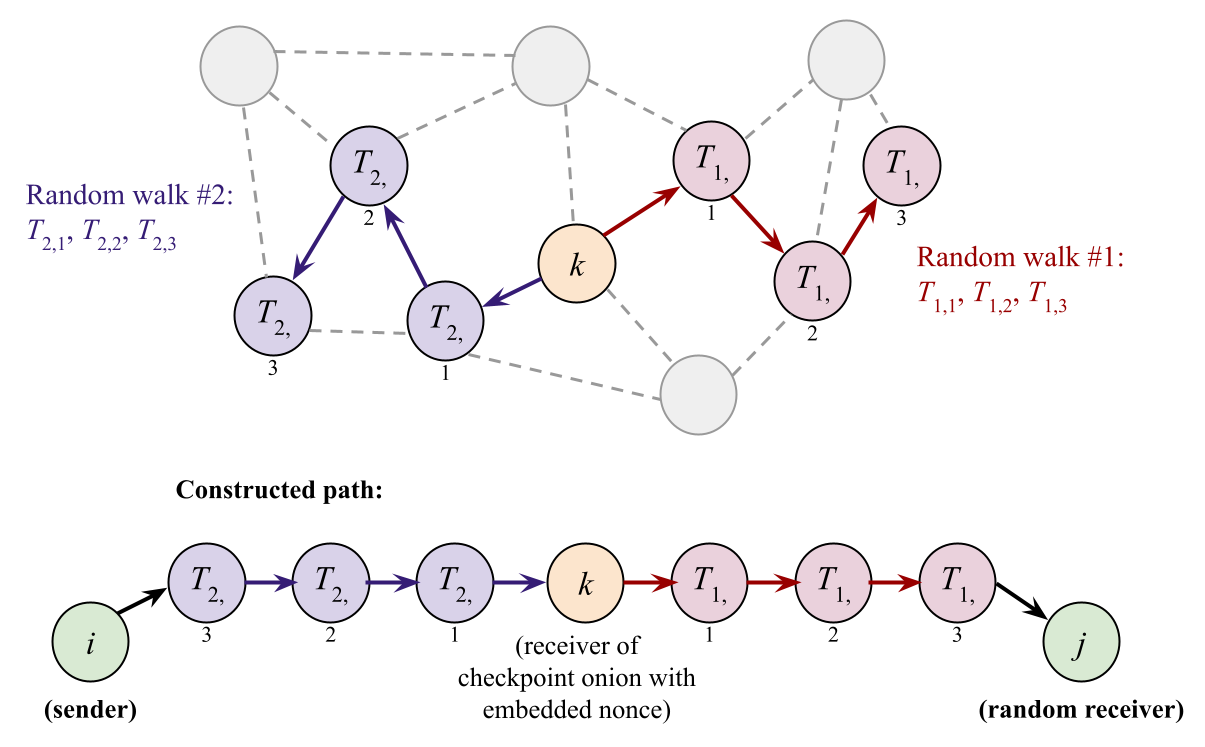
\includegraphics[width=400pt]{template/figures/constructing-checkpoint-onion-path.png}
\end{center}
 
\textbf{\textit{Routing.}} Assume a sender $i$ forms a dummy onion with a nonce $s_{\frac{L}{2}}$ embedded in the $\frac{N}{2}$-th layer, and assume $k$ is an honest party intended to receive this onion in round $\frac{L}{2}$. Then $k$ should also receive a symmetric dummy onion formed by some other sender $h$, such that when the onion is processed, it reveals the same nonce $s_{\frac{L}{2}}$. After $k$ peels all its onions in round $\frac{N}{2}$, it counts the number of unmatched checkpoint nonces. If this count exceeds a threshold value $t$, then $k$ knows to abort the protocol run; otherwise, at round $\frac{n}{2} + 1$, the peeled onions are sent to their next destinations in random order.\\

\textbf{\textit{Correctness and efficiency.}} Recalling that correctness is defined with respect to the passive adversary, $\Pi_x$ is clearly correct. Moreover, unless an honest party aborts the protocol run, all messages that are not dropped by the adversary are delivered to their final destinations. In $\Pi_x$, the communication complexity blow-up is $O(\log^6 \lambda)$, since the latency is $L+1 = O(\log^2 \lambda)$ rounds, and the server load is $O(\log^4 \lambda)$.\\\\
\textbf{\textit{Privacy.}} To prove that $\Pi_x$ is secure, we require that the thresholding mechanism does its job:

\begin{theorem} \label{clm:active}
    For any constant $\epsilon > 0$, with parameters $L = \Omega(\text{polylog }\lambda)$ and $t = O(\log^2 \lambda)$, $\Pi_x$ is computationally $(\epsilon, \text{negl}(\lambda))$-differentially private from the adversary who corrupts up to $\chi < \frac{1}{2}$ fraction of the parties and drops any fraction $0 \leq \gamma \leq 1$ of the indistinguishable onions.\\
\end{theorem}

\begin{proof} [Proof of Theorem~\ref{clm:active}]
We prove below that $\Pi_x$ achieves (statistical) $(\epsilon, \text{negl}(\lambda))$-differential privacy for any constant $\epsilon > 0$ when the PRF $F$ is truly a random function.\\

Let $\sigma_0, \sigma_1$ be any neighboring input vectors. That is, $\sigma_0$ and $\sigma_1$ are identical except on the inputs of two honest senders $P_i$ and $P_j$ and the ``outputs'' of two receivers $P_u$ and $P_v$. On input vector $\sigma_0$, $P_i$ sends a message to $P_v$; while in $\sigma_1$, this is swapped ($P_i$ sends to $P_v$, while $P_j$ sends to $P_u$). For $b \in \{0, 1\}$, let $(I_{i,1}, \dots, I_{i,\ell_1+\ell_2}, R_{b,i})$ be the routing path that $P_i$ picks for their message-bearing onion, and let $(I_{j,1}, \dots, I_{j,\ell_1+\ell_2}, R_{b,j})$ be the routing path that $P_j$ picks for their message-bearing onion.\\

We prove the theorem by cases.\\

\textbf{Case 1:} \textit{neither $P_i$'s message nor $P_j$'s message is delivered}. The adversarial views for the two settings are perfectly indistinguishable since the adversary never observes the onions' layers for $P_u$ and $P_v$, i.e., $\text{View}_{\Pi_x^{\mathcal{A}}}(\sigma_0) = \text{View}_{\Pi_x^{\mathcal{A}}}(\sigma_1)$.\\

\textbf{Case 2:} \textit{both $P_i$'s message and $P_j$'s message is delivered}. In this case, $\text{View}_{\Pi_x^{\mathcal{A}}}(\sigma_0)$ is statistically indistinguishable from $\text{View}_{\Pi_x^{\mathcal{A}}}(\sigma_1)$, by Theorem \ref{clm:passive}.\\

\textbf{Case 3:} \textit{either $P_i$'s or $P_j$'s message is delivered, and the other is dropped}. In this case, we will prove that $\text{View}_{\Pi_x^{\mathcal{A}}}(\sigma_0)$ and $\text{View}_{\Pi_x^{\mathcal{A}}}(\sigma_1)$ are differentially private. W.l.o.g., we assume that $P_i$'s message makes it to its recipient $R_{b,i}$, but $R_{b,j}$ does not receive $P_j$'s message. The only information the adversary has to help determine the input setting is the volumes of onions received by each recipient. W.o.p., the number $n$ of indistinguishable checkpoint onions for either $P_u$ or $P_v$ is arbitrarily close to the expected number $\mathbb{E}[n]$ (since $\mathbb{E}[n]$ is polylogarithmic in the security parameter). Seen this way, the number of indistinguishable checkpoint onions for $P_u$, which we denote by $n_u$, and the number of indistinguishable checkpoint onions for $P_v$, which we denote by $n_v$, are Binomial random variables with $n$ trials and bias $\frac{1}{2}$, i.e., $n_u, n_v \sim \text{Binomial}(n, \frac{1}{2})$. Thus, the numbers of messages received are obscured by a Binomial Mechanism which, for $n = \Omega(\text{polylog } \lambda)$, was shown~\cite{EC:DKMMN06} to be $(\epsilon/2, \text{negl}(\lambda))$-differentially private for any positive constant $\epsilon$. It follows from the composition theorem for differential privacy that $\Pi_x$ achieves (computational) $(\epsilon, \text{negl}(\lambda))$-differential privacy for any positive constant $\epsilon$. 

\end{proof}

\newpage

 

\section{Our Protocol: Wrapping Onions} \label{sec:woes}

\subsection{Overview}

At a high level, the wrapping onions protocol begins just like traditional onion routing: a client forms an onion by encrypting a message with multiple layers of encryption. Each relay in the path is chosen uniformly at random from all available nodes without regard for the underlying topology. 

Let's say for some sender, receiver pair $(S, R)$, $S$ forms an onion $O = (O_1, O_2,..., O_{L+1})$ with routing path $(P_1, P_2,...,P_L, R)$, where $L = \Omega(\log \lambda)$ denotes the static nodes in the path. For each round $i \leq L$, When $P_i$ receives $O_i$ and peels off its outer layer to reveal $O_{i+1}$, it learns the identity of the next intended hop, $P_{i+1}$. Then, using its knowledge of the current network topology, for some detour length $d = \Omega(\log \lambda)$, the node $P_i$ determines an intermediate path $(P_{i,1}, P_{i,2},..., P_{i,d})$, where $P_{i,d}$ is some direct neighbor of $P_{i+1}$. Asume this path is chosen uniformly at random from all possible paths from $P_i$ to $P_{i+1}$. Then, $P_i$ uses this path to wrap $O_{i+1}$ in $d$ additional layers of encryption, forming a new onion,
$$
O_i' \leftarrow \texttt{FormOnion}(O_{i+1}, (P_{i,1}, P_{i,2},..., P_{i,d}), (pk_{i,1}, pk_{i,2},..., pk_{i,d}))
$$ 
$$
= (O_{i,1}, O_{i,2}, ..., O_{i,d}, O_{i+1}),
$$
so that after $d$ rounds, $P_{i,d}$ will peel $O_{i+1,d}$, revealing $O_{i+1}$ to be sent directly to $P_{i+1}$. 

\begin{center}
    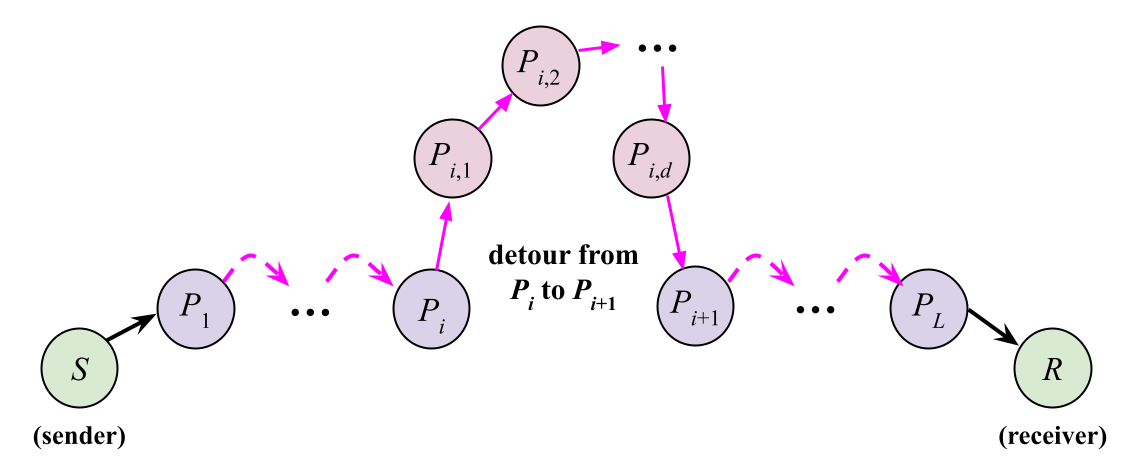
\includegraphics[width=375pt]{template/figures/detour.png}
\end{center}
Note that with $L, d = \Omega(\log \lambda)$, the total path length will be $\Omega(\log^2 \lambda)$

\subsection{Correctness}



\subsection{Resilience to Churn}

Another advantage of the wrapping onions approach is its resilience to network churn. Previously, if even a single node in the predetermined path goes offline, the onion may become ``stuck'' with no valid route to its destination. In the wrapping onions model, only the $L$ nodes chosen initially by the client need to be online for the entirety of the protocol. The detours and network topology (connections between nodes) can be adjusted dynamically. 

\clearpage

\subsection{Parameters}

Let $l = \Omega(\log \lambda)$ represent the initial path length constructed by the client sender. Denote $d = \Omega(\log \lambda)$ as the length of each detour. Then $L = ld = \Omega(\log^2 \lambda)$ represents the total path length from sender to receiver.

\subsection{Privacy Guarantees}

\subsubsection{Passive Adversary}

\begin{theorem} \label{clm:passive-2}
    $\Pi_w$ is statistically private against a passive adversary who can monitor up to a constant fraction $\chi < \frac{1}{2}$ of the servers. Assume $\frac{N}{n} = \Omega(\log^2 \lambda)$ and $d = \Omega(\log \lambda)$, $L = \Omega(\log^2 \lambda)$, where $\lambda \in \mathbb{N}$ represents the security parameter.\\
\end{theorem}

\begin{proof} [Proof of Theroem~\ref{clm:passive-2}]
    
\end{proof}


\subsection{Communication Complexity Blow-up}

\subsubsection{Packet Size}

\subsubsection{Latency}




\section{Conclusion and Open Problems}


\clearpage
% ~~~ REFERENCES ~~~ %
%\bibliographystyle{plain}
%\bibliographystyle{is-alpha}
\bibliographystyle{stylefiles/alpha-short}
\bibliography{template/bibfiles/abbrev3,template/bibfiles/crypto,template/bibfiles/anon,template/bibfiles/refs} 

\appendix 

\clearpage

% MORE PROOFS
\section{Supplementary proofs} \label{sec:proofs}

\begin{lemma} \label{lem:chernoff} Consider a random experiment with $n$ equally likely outcomes conducted over $N$ independent Poisson trials. For sufficiently large $n$, if $N = \omega(n \log n)$, then every outcome occurs a number of times arbitrarily close to its expected value, $\frac{N}{n}$. 
\end{lemma} 

\begin{proof}[Proof of Lemma~\ref{lem:chernoff}]
Let $X_i$ denote the number of times some outcome $i \in [n]$ occurred after $N$ trials. Then $\mathbb{E}[X_i]$ = $\frac{N}{n}$, and it follows from Chernoff bounds~\cite[Cor.~4.6]{MU05} that for all $0 < \delta < 1$:
$$
\Pr\left(|X - \frac{N}{n}| \geq \delta \cdot \frac{N}{n} \right) \leq 2 e^{-\frac{\delta^2 \cdot N}{3n}}.
$$
Applying the union bound over all $n$ outcomes, we get:
$$
\Pr\left(\exists i \in [n]: |X - \frac{N}{n}| \geq \delta \cdot \frac{N}{n} \right) \leq n \cdot 2 e^{-\frac{\delta^2 \cdot N}{3n}} = 2 e^{\ln n -\frac{\delta^2 \cdot N}{3n}}.
$$
Substituting $N = \omega(n \log n)$, we can simplify the expression in the exponent:
$$
\ln n - \frac{\delta^2 \cdot \omega(n \log n)}{3n} = \omega(-\log n).
$$
Since $e^{\omega(-\log n)}$ decays to 0 as $n \rightarrow \infty$, it follows that the probability that any outcome occurs significantly more or less than the expected value, $\frac{N}{n}$, is negligible for sufficiently large $n$.
\end{proof}


\begin{lemma} \label{lem:chernoff-1} Consider the same setup as in Lemma~\ref{lem:chernoff}, but now we express $n$ and $N$ as functions of the security parameter $\lambda$. If $N = \mathsf{poly}(\lambda)$ and $n = O(N / \log^\epsilon \lambda)$ for all $\epsilon \geq 2$, then every outcome occurs a number of times arbitrarily close to the expected value, $\frac{N}{n}$, with overwhelming probability in $\lambda$.
\end{lemma} 

\begin{proof}[Proof of Lemma~\ref{lem:chernoff-1}]

For $N = \mathsf{poly}(\lambda)$ and $n = O(N / \log^\epsilon \lambda)$, we can write:
$$
n \log n = O\left(\frac{\mathsf{poly}(\lambda)}{\log^\epsilon \lambda} \cdot \log\left(\frac{\mathsf{poly}(\lambda)}{\log^\epsilon \lambda}\right)\right) = o(\mathsf{poly}(\lambda)).
$$
Thus,
$$
N = \mathsf{poly}(\lambda) = \omega(n \log n).
$$
Applying Lemma~\ref{lem:chernoff}, we conclude that every outcome occurs a number of times arbitrarily close to the expected value, $\frac{N}{n}$. 
\end{proof}

\begin{lemma} \label{lem:chernoff-2} Continuing the result from Lemma~\ref{lem:chernoff-1}, it follows that any subset of $k$ outcomes (where $k \in [n]$) will occur a number of times arbitrarily close to the expected value $\frac{kN}{n}$, with overwhelming probability in $\lambda$.
\end{lemma} 

\begin{proof}[Proof of Lemma~\ref{lem:chernoff-2}]
Let $S$ denote a subset of $k$ outcomes, and let $O_S$ represent the total number of trials that resulted in one of these outcomes, with an expected value of $\mathbb{E}[O_S] = \frac{kN}{n}$. Now assume, for the sake of contradiction, that with non-negligible probability, $O_S$ differs from the expectation by more than a positive factor $\delta < 1$.

Then by the pigeonhole principle, there is a non-negligible probability that at least one outcome occurred significantly more or less times than $\frac{N}{n}$. However, this contradicts Lemma \ref{lem:chernoff-2}. Thus, the probability must be negligible in $\lambda$.
\end{proof}

\end{document}